% !TEX root = _individual/implementation.tex

%%%%%%%%%%%%%%%%%%%%%%%%%%%%%%%%%%%%%%%%%%%%%%%%%%%%%%%%%%%%%%%%%%%%%%%%%%%%%%%%
\chapter{Low-order discretization schemes} \label{chap:implementation}

Tensor diffusion---the diffusion of particles through anisotropic fields---has
many applications outside of our work, including the fields of geology,
magnetohydrodynamics, and image reconstruction. Numerous tensor diffusion
schemes have been developed, but many of these are more general than we need in
our work. The anisotropic diffusion tensor derived in
Chapter~\ref{chap:adDerivation} is relatively well behaved: it is a smooth
function in space, it tends toward isotropy in optically thick problems, it is
SPD, it is diagonally dominant, and so forth. Additionally, our test problems
are executed in a structured
two-dimensional Cartesian mesh: all cells are quadrilaterals, and each
interior cell to four adjacent cells through four faces, and each face is
perpendicular to one of the coordinate system axes.

Because of these simplifying properties, we need not use some of the more
complex discretization schemes, which tend to have higher numbers of unknowns
per spatial cell and are therefore more costly to solve.
(An example is the Support Operators Method \cite{Mor1998,Run2006}, with
roughly three unknowns per cell.) Instead, we derive some simple
finite volume discretization schemes for anisotropic diffusion. Because the
boundary conditions for our AD method are distinct from standard diffusion
boundary conditions, we also present a second-order-accurate discretization of
them.

The ``Anisotropic \Pone'' scheme is entirely new, so we develop a discretization
scheme for it by making a minor modification to the traditional \Pone\
discretization: a
``staggered mesh'' where $\phi$ is cell-centered and $\vec{F}\vd \vec{n}$ is
stored on the edges of each cell \cite{War2003}.
% This approach conserves radiation energy, but it does not conserve radiation
% momentum, an important quantity when coupling with hydrodynamics codes
% \cite{Pom1973}.

%%%%%%%%%%%%%%%%%%%%%%%%%%%%%%%%%%%%%%%%%%%%%%%%%%%%%%%%%%%%%%%%%%%%%%%%%%%%%%%%
\section{Introduction}

Because the semi-implicit gray TRT formulation of the particle conservation
equation can be expressed as a steady-state transport equation (see
\S\ref{sec:bgSemiImplicit}), for the sake of simplicity we will present the
anisotropic diffusion discretizations without time dependence.

The steady-state particle conservation equation is
\begin{equation}\label{eq:ssConservation}
  \grad \vd \vec{F}(\vec{x}) + \sigma_a(\vec{x}) \phi(\vec{x}) =
  Q(\vec{x})\,,\qquad \vec{x} \in V\,.
\end{equation}
(In an implicitly discretized time-dependent problem,
$\vec{F}=\vec{F}(t^{n+1})$, $\phi=\phi(t^{n+1})$, $\sigma_a$ is modified from
the true absorption opacity by adding $\frac{1}{c\Delta_t}$, and the source $Q$
contains an additional $\frac{\phi(t^{n})}{c\Delta_t}$.) 

The first step in a finite volume scheme is to assume that the unknown---%
in this case, $\phi$---is constant over a single cell, represented in
Fig.~\ref{fig:cellDiagram}. 
%
\begin{figure}[tb]
  \centering
  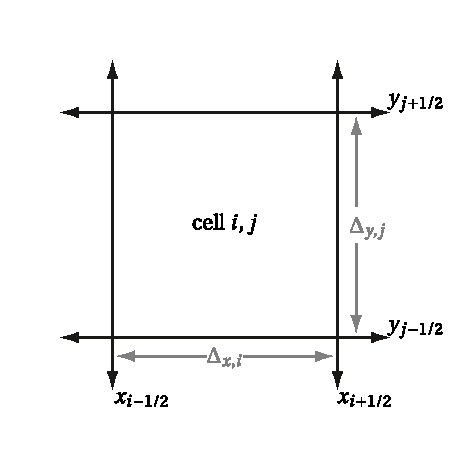
\includegraphics{cell-diagram}
  \caption{Diagram of cell $i,j$.}
  \label{fig:cellDiagram}
\end{figure}
%
We also assume that the effective absorption opacity $\sigma_a$ and source $Q$
are
constant over the cell, which, for TRT, means assuming the material temperature
is constant over a cell. Integrating Eq.~\eqref{eq:ssConservation} over cell
$i,j$ and using the divergence theorem gives
\begin{equation} \label{eq:ssConservationDisc}
  %\sum_{f\in \{L,R,B,T\}} \int_f \vec{n}_f \vd \vec{F} \ud A
  \Delta_{x,i} \left( F_T^y - F_B^y \right)
+ \Delta_{y,j} \left( F_R^x - F_L^x \right)
+ \Delta_{x,i}\Delta_{y,j} \sigma_{a,i,j} \phi_{i,j}
= \Delta_{x,i}\Delta_{y,j} q_{i,j}\,.
\end{equation}
Here, $F_A^b$ is the leakage (i.e., radiation flux or particle flow rate) from
cell $i,j$ through face $A$
along the $b$ axis.In all discretizations of the conservation equation, it is essential that
$\vec{F}$ be continuous at cell interfaces: e.g., $F_T^y$ from cell $i,j$ must
be equal to -$F_B^y$ from cell $i,{j+1}$.

The methods presented in the following sections provide different
approximate closures for the leakages in terms of the other unknowns.
In the case of anisotropic diffusion, the leakages are determined by the
anisotropic Fick's law:
\begin{equation}\tagref{eq:adFicks}
  \vec{F}(\vec{x}) = - \Dtens(\vec{x}) \vd \grad \phi(\vec{x}) \,.
\end{equation}
With the anisotropic \Pone\ approximation, Fick's law is replaced by the \APone\
equation:
\begin{equation}\tagref{eq:ap1FicksLawFinal}
  \frac{1}{c}\pder{\vec{F}}{t}(\vec{x},t)
  + \varsigma(\vec{x}) \Dtens(\vec{x}) \vd \grad \phi(\vec{x}, t)
  + \varsigma(\vec{x})\vec{F}(\vec{x},t) 
  = 0 \,.
\end{equation}
Discretizing this equation implicitly in time and solving for $\vec{F}$, we
obtain:
\begin{subequations}\label{eqs:ap1FicksImplicit}
\begin{equation}\label{eq:ap1FicksImplicit}
  \vec{F}(\vec{x}) = - [1 - \eta(\vec{x})]\Dtens(\vec{x}) \vd \grad \phi(\vec{x})
  + \eta(\vec{x}) \hat{\vec{F}}(\vec{x})\,,
\end{equation}
where $\vec{F} = \vec{F}(t^{n+1})$, $\hat{\vec{F}}=\vec{F}(t^n)$, and
\begin{equation}\label{eq:ap1ImplicitEta}
  \eta(\vec{x}) \equiv \frac{1}{1 + \varsigma(\vec{x}) c \Delta_t}\,.
\end{equation}
\end{subequations}
Setting $\eta=0$ reduces this equation to Eq.~\eqref{eq:adFicks2d}.

Equation~\eqref{eq:ap1FicksImplicit} in 2-D comprises two equations in vector
form:
\begin{align}\label{eq:ficks2d}
  \begin{bmatrix}
    F^{x} \\
    F^{y}
  \end{bmatrix}
  &= - (1 - \eta)
  \begin{bmatrix}
    D^{xx} & D^{yx} \\
    D^{xy} & D^{yy}
  \end{bmatrix}
  \begin{bmatrix}
    \tpder{\phi}{x} \\
    \tpder{\phi}{y}
  \end{bmatrix}
  + \eta
  \begin{bmatrix}
    \hat{F}^{x} \\
    \hat{F}^{y}
  \end{bmatrix}
  \\ \nonumber
  &= 
  \begin{bmatrix}
    - (1 - \eta)D^{xx} \tpder{\phi}{x}
    - (1 - \eta)D^{yx} \tpder{\phi}{y}
    + \eta \hat{F}^{x}
    \\
    - (1 - \eta)D^{yy} \tpder{\phi}{y}
    - (1 - \eta)D^{xy} \tpder{\phi}{x}
    + \eta \hat{F}^{x}
  \end{bmatrix}
\end{align}
The diagonal components of $\Dtens$ contribute to ``normal''
leakage; and the off-diagonal components $D^{xy}$ contribute to ``transverse''
leakage, particle movement across the face due to a gradient in the transverse
direction.
Note that since the anisotropic diffusion tensor is symmetric,
$D^{yx}=D^{xy}$.

Setting $\eta=0$ results in the simpler anisotropic diffusion representation:
\begin{equation}\label{eq:adFicks2d}
  \begin{bmatrix}
    F^{x} \\
    F^{y}
  \end{bmatrix}
  = -
  \begin{bmatrix}
    D^{xx} & D^{yx} \\
    D^{xy} & D^{yy}
  \end{bmatrix}
  \begin{bmatrix}
    \tpder{\phi}{x} \\
    \tpder{\phi}{y}
  \end{bmatrix}
  = 
  \begin{bmatrix}
    - D^{xx} \tpder{\phi}{x}
    - D^{yx} \tpder{\phi}{y}
    \\
    - D^{yy} \tpder{\phi}{y}
    - D^{xy} \tpder{\phi}{x}
  \end{bmatrix}
\end{equation}

%%%%%%%%%%%%%%%%%%%%%%%%%%%%%%%%%%%%%%%%%%%%%%%%%%%%%%%%%%%%%%%%%%%%%%%%%%%%%%%%
\section{Neglecting transverse diffusion}\label{sec:discreteDiag}

Perhaps the simplest way to discretize the anisotropic equations in
structured Cartesian geometry is to neglect the off-diagonal terms of the
diffusion tensor that cause transverse leakage.
In certain simple problems, this is not an approximation. As long as the
opacity is invariant with respect to one of the Cartesian coordinate system's
axes (see \S\ref{sec:adVoids}), the off-diagonal terms of $\Dtens$ are
identically zero.

%%%%%%%%%%%%%%%%%%%%%%%%%%%%%%%%%%%%%%%%
\subsection{Anisotropic diffusion}
Setting $D^{yx}=D^{xy}=0$ simplifies Eq.~\eqref{eq:adFicks2d} to:
\begin{equation*}
  \begin{bmatrix}
    F^{x} \\
    F^{y}
  \end{bmatrix}
  = -
  \begin{bmatrix}
    D^{xx} & 0 \\
    0 & D^{yy}
  \end{bmatrix}
  \begin{bmatrix}
    \tpder{\phi}{x} \\
    \tpder{\phi}{y}
  \end{bmatrix}
  = 
  \begin{bmatrix}
    - D^{xx} \tpder{\phi}{x} \\
    - D^{yy} \tpder{\phi}{y}
  \end{bmatrix}
  \,.
\end{equation*}

Without loss of generality, we evaluate the net leakage from cell
$i,j$ through its right face, which has an outer normal along the $+x$ axis,
$\vec{n}_R = [1,0]$:
\begin{align} \nonumber
  F_R^x &\equiv \frac{1}{\Delta_{y,j}} \int_{y_{j-1/2}}^{y_{j+1/2}}
  \vec{F}(x_{i+1/2}, y) \vd \vec{n}_R \ud y\,.
  \\
  \intertext{Substituting the anisotropic Fick's law, we obtain} \nonumber
  F_R^x &= - \frac{1}{\Delta_{y,j}} \int_{y_{j-1/2}}^{y_{j+1/2}}
  D_{i,j}^{xx} \pder{\phi}{x} \ud y \,.
  \\ 
  \intertext{Now we introduce a temporary cell-edge $\phi_*$ to
  approximate the partial derivative using a second-order finite difference
  stencil:}
  \label{eq:diagFrx}
  F_R^x &\approx - 
  D_{i,j}^{xx} \frac{\phi_* - \phi_{i}}{\Delta_{x,i}/2} \,.
\end{align}

Now we evaluate the leakage on the same face in the same $+x$ direction, but
from the perspective of cell $i+1,j$. Approximating the derivative using the
same cell-edged $\phi_*$, we obtain
\begin{equation}\label{eq:diagFlx}
  F_{L,i+1,j}^x \approx - 
  D_{i+1,j}^{xx} \frac{\phi_{i+1,j} - \phi_*}{\Delta_{x,i+1}/2} \,.
\end{equation}
Scaling Eqs.~\eqref{eq:diagFrx} and~\eqref{eq:diagFlx} by $\Delta_x/(2 D^{xx})$
and adding them, we obtain
\begin{equation*}
  \frac{\Delta_{x,i+1}/2}{D_{i,j}^{xx}}F_R^x
 + \frac{\Delta_{x,i+1}/2}{D_{i+1,j}^{xx}}F_{L,i+1,j}^x
 = -(\phi_* - \phi_{i}) + -(\phi_{i+1,j} - \phi_*)\,.
\end{equation*}
The temporary cell-edged $\phi_*$ is eliminated. Now we enforce particle
conservation by setting $F_{L,i+1,j}^x = F_R^x$ and solve for $F_R^x$. This
gives the following expression for the net leakage through the right face of
cell $i,j$:
\begin{equation}\label{eq:diagRight}
  F_R^x= -\frac{D^{xx}_{i+1/2,j}}{\Delta_{x,i+1/2}}
  \left( \phi_{i+1,j} - \phi_{i,j} \right)\,,
\end{equation}
where we have defined a harmonically averaged cell edge diffusion coefficient
and a half-edge width,
\begin{equation} \label{eq:cellEdgeDHarmonic}
  \frac{D^{xx}_{i+1/2,j}}{\Delta_{x,i+1/2}} \equiv \left[
  \frac12 \left( \frac{D^{xx}_{i,j}}{\Delta_{x,i}} \right)\inv
 + \frac12 \left( \frac{D^{xx}_{i+1,j}}{\Delta_{x,i+1}} \right)\inv
  \right]\inv\,.
\end{equation}
This is the standard relation between neighboring cells in the
cell-centered discretization scheme \cite{Dud1976}, except that in anisotropic
diffusion, leakage across the face normal to the $x$ axis takes the $D^{xx}$
component of the diffusion tensor.

The same procedure yields similar for the three other faces of cell $i,j$:
\begin{align*}
  F_L^x &= -\frac{D^{xx}_{i-1/2,j}}{\Delta_{x,i-1/2}}
  \left( \phi_{i,j} - \phi_{i-1,j} \right)\,,
  \\
  F_T^y &= -\frac{D^{yy}_{i,j+1/2}}{\Delta_{y,j+1/2}}
  \left( \phi_{i,j+1} - \phi_{i,j} \right)\,,
  \\
  F_B^y &= -\frac{D^{yy}_{i,j-1/2}}{\Delta_{y,j-1/2}}
  \left( \phi_{i,j} - \phi_{i,j-1} \right)\,.
\end{align*}
These terms, substituted into Eq.~\eqref{eq:ssConservationDisc}, relate the
cell-centered values of $\phi$ in the interior:
\begin{multline} \label{eq:diagConservation}
  \hphantom{ {}+{} }
  \Delta_{x,i} \left(
  - \frac{D^{yy}_{i,j+1/2}}{\Delta_{y,j+1/2}} \left( \phi_{i,j+1} - \phi_{i,j}
    \right)
  + \frac{D^{yy}_{i,j-1/2}}{\Delta_{y,j-1/2}} \left( \phi_{i,j} - \phi_{i,j-1}
    \right)
  \right)
\\
\shoveleft{%
  {}+ \Delta_{y,j} \left(
  - \frac{D^{xx}_{i+1/2,j}}{\Delta_{x,i+1/2}} \left( \phi_{i+1,j} - \phi_{i,j}
    \right)
  + \frac{D^{xx}_{i-1/2,j}}{\Delta_{x,i-1/2}} \left( \phi_{i,j} - \phi_{i-1,j}
    \right)
  \right)
}
\\
{}+ \Delta_{x,i}\Delta_{y,j} \sigma_{a,i,j} \phi_{i,j}
= \Delta_{x,i}\Delta_{y,j} q_{i,j}\,.
\end{multline}
Rearranging shows the leakage terms to be part of a discretized Laplacian
operator.

When a cell has one or more face on an exterior boundary, the above relations
for $\vec{n}\vd \vec{F}$ are replaced by a discretized form of the boundary
condition, which we shall derive presently.

%%%%%%%%%%%%%%%%%%%%%%%%%%%%%%%%%%%%%%%%
\subsection{Anisotropic \texorpdfstring{\Pone}{P1}}

The time-dependent \Pone\ and anisotropic \Pone\ methods require the radiation
flux $\vec{F}$ to be stored along side the scalar intensity $\phi$. Using the
same finite differencing procedure as performed above for anisotropic diffusion,
we obtain a discretization for \APone\ that stores $\phi$ in cell centers and
$\vec{F}$ on cell edges.
%Because the locations of the cell edges are distinct
%from the cell centers, this is known as a ``staggered grid'' approximation
%\cite{War2003}.
In the steady-state case, this discretization reduces to the above anisotropic
diffusion discretization.

We evaluate the 2-D anisotropic \Pone\ equation~\eqref{eq:ficks2d} on the right
face of cell $i,j$, set $D^{yx}=0$, and introduce the temporary cell-edge
$\phi_*$ to approximate the derivative normal to the face:
\begin{equation*}
  F_{i+1/2,j}^{x} =
  - (1 - f_{i,j})D_{i,j}^{xx} \frac{\phi_* - \phi_{i,j}}{\Delta_{x,i}/2}
  + f_{i,j} \hat{F}_{i+1/2,j}^{x} \,.
\end{equation*}
Evaluating the leakage on same face from cell $i+1,j$, we obtain:
\begin{equation*}
  F_{i+1/2,j}^{x} =
  - (1 - f_{i+1,j})D_{i+1,j}^{xx} \frac{\phi_{i+1,j} - \phi_*}{\Delta_{x,i+1}/2}
  +  f_{i+1,j} \hat{F}_{i+1/2,j}^{x} \,.
\end{equation*}
Multiplying the equations by $(\Delta_{x} / 2) / [(1 - \eta) D^{xx}]$, we eliminate
the temporary $\phi_*$:
\begin{subequations}\label{eqs:diagApone}
\begin{multline}\label{eq:diagAponeX}
  \left[
    \frac{\Delta_{x,i}/2}{(1 - f_{i,j})D_{i,j}^{xx}}
  + \frac{\Delta_{x,i+1}/2}{(1 - f_{i+1,j})D_{i+1,j}^{xx}} \right]
  F_{i+1/2,j}^{x}
  \\ = \phi_{i,j} - \phi_{i+1,j}
  + \left[
    \frac{f_{i,j} \Delta_{x,i}/2}{(1 - f_{i,j})D_{i,j}^{xx}}
  + \frac{f_{i+1,j} \Delta_{x,i+1}/2}{(1 - f_{i+1,j})D_{i+1,j}^{xx}}
  \right] \hat{F}_{i+1/2,j}^{x}  \,.
\end{multline}
For faces normal to the $y$ axis, the corresponding equation is:
\begin{multline}\label{eq:diagAponeX}
  \left[
    \frac{\Delta_{y,j}/2}{(1 - f_{i,j})D_{i,j}^{yy}}
  + \frac{\Delta_{y,j+1}/2}{(1 - f_{i,j+1})D_{i,j+1}^{yy}} \right]
  F_{i,j+1/2}^{y}
  \\ = \phi_{i,j} - \phi_{i,j+1}
  + \left[
    \frac{f_{i,j} \Delta_{y,j}/2}{(1 - f_{i,j})D_{i,j}^{yy}}
  + \frac{f_{i,j+1} \Delta_{y,j+1}/2}{(1 - f_{i,j+1})D_{i,j+1}^{yy}}
  \right] \hat{F}_{i,j+1/2}^{y}  \,.
\end{multline}
\end{subequations}

Equations~\eqref{eqs:diagApone} relate the flux at a face with the scalar
intensity in the adjacent cells. They provide one equation for each interior
face; the conservation equation~\eqref{eq:ssConservationDisc} provides an
equation for each cell; and a discretization of the anisotropic \Pone\ boundary
conditions provides an equation for each boundary face.

%%%%%%%%%%%%%%%%%%%%%%%%%%%%%%%%%%%%%%%%%%%%%%%%%%%%%%%%%%%%%%%%%%%%%%%%%%%%%%%%
\subsection{Boundary conditions}

The specified incident boundary condition for anisotropic diffusion is given in
Eq.~\eqref{eq:loBc}:
\begin{equation*}
2\int_{\vec{\Omega}\vd\vec{n} < 0} W(\abs{\vec{\Omega}\vd\vec{n}})
I^b \ud\Omega
=
\phi
+ 2 \vec{d} \vd \grad \phi\,,
\end{equation*}
where the boundary coefficient is given in Eq.~\eqref{eq:adBoundaryIntegral}:
\begin{equation*}
  \vec{d} = -\int_{\vec{\Omega}\vd\vec{n} < 0} W(\abs{\vec{\Omega}\vd\vec{n}})
\vec{\Omega} \eta \ud\Omega\,.
\end{equation*}

The anisotropic \Pone\ boundary condition, Eq.~\eqref{eq:ap1BoundaryCondition}
is similar:
\begin{equation*}
  2 \int_{\vec{\Omega}\vd\vec{n} < 0}
  W(\abs{\vec{\Omega}\vd\vec{n}}) I^b \ud\Omega
  = \phi
  - 2 \vec{d} \vd \Dtens\inv \vd \vec{F} \,,
\end{equation*}
where $\vec{d}$ is the same as in anisotropic diffusion.
In fact, by substituting the time-discretized $\vec{F}$ from
Eq.~\eqref{eq:ap1FicksImplicit}, we obtain a general boundary condition that
reduces to the anisotropic diffusion boundary condition by setting $\eta=0$:
\begin{align*}
  2 \int_{\vec{\Omega}\vd\vec{n} < 0}
  W(\abs{\vec{\Omega}\vd\vec{n}}) I^b \ud\Omega
  &= \phi
  - 2 \vec{d} \vd \Dtens\inv \vd 
  \left[ - (1 - \eta)\Dtens \vd \grad \phi + \eta \hat{\vec{F}} \right]
  \\
  &=  \phi + 2 (1 - \eta) \vec{d} \vd \grad \phi
  - 2 \eta \vec{d} \vd \Dtens\inv \vd \hat{\vec{F}} \,.
\end{align*}

Looking ahead to using flatland geometry as well as 2-D, we write this
AD/\APone\ boundary condition as:
\begin{equation}\label{eq:discreteBcGeneral}
  q = \phi + r (1 - \eta) \vec{d} \vd \grad \phi
  - r \eta \vec{d} \vd \Dtens\inv \vd \hat{\vec{F}}\,,
\end{equation}
where $q$, $r$, $\vec{d}$, and $\Dtens$ all depend upon the chosen geometry. The
values $q$ and $r$ are given in Table~\ref{tab:discreteBcCoeffs}.

\begin{table}[tb]
  \centering
  \begin{tabular}{rcc}
\toprule
& $q$
& $r$
\\ \midrule
1-D/2-D/3-D
& $2 \int_{\vec{\Omega}\vd\vec{n} < 0}
  W(\abs{\vec{\Omega}\vd\vec{n}}) I^b \ud\Omega$
  & $2\vphantom{\Big|}$
\\
Flatland
& $2 \pi \int_{\vec{\Omega}\vd\vec{n} < 0}
  V(\abs{\vec{\Omega}\vd\vec{n}}) I^b \ud\Omega$
& $\pi/2\vphantom{\Big|}$
\\ \bottomrule
  \end{tabular}
  \caption[Coefficients for the discretized boundary conditions.]{%
    Coefficients for the discretized boundary conditions. The flatland values
    and the function $V$ are discussed in Chapter~\ref{chap:flatland}. }
  \label{tab:discreteBcCoeffs}
\end{table}

At this point, Eq.~\eqref{eq:discreteBcGeneral} is very general: it applies not
just to Cartesian geometries, and it does not depend on the assumption that
$D^{yx}=D^{xy}=0$. Now we make the analysis slightly less specific by demanding
that $\eta$ be azimuthally symmetric about the outward normal of the boundary face.
(Equivalently, we discard the $D^{yx}=D^{xy}$ terms if the boundary face is
along one of the coordinate axes.) With this assumption, as discussed in
\S\ref{sec:adLinalg}, the normal vector is an eigenvector of $\Dtens$:
\begin{equation*}
  \Dtens \to D \vec{n}\vec{n}\,,
\end{equation*}
and the boundary coefficient is pointed along the outward normal:
\begin{equation*}
  \vec{d} \to d \vec{n}\,.
\end{equation*}

Under this assumption, Eq.~\eqref{eq:discreteBcGeneral} simplifies greatly
(using the fact that $\vec{n}$ is a unit vector):
\begin{align} \nonumber
  q &= \phi + r (1 - \eta) \left[ d \vec{n} \right] \vd \grad \phi
  - r \eta \left[ d \vec{n} \right] \vd \left[ D \vec{n}\vec{n} \right] \vd
  \hat{\vec{F}}\,,
  \\ \label{eq:discreteBcGeneralQ}
 q &=  \phi + (1 - \eta) dr \vec{n} \vd \grad \phi
  - \frac{\eta dr}{D} \hat{F} \,,
\end{align}
where we have defined the outward component of the previous time step's
radiation flux as
\begin{equation*}
  \hat{F} \equiv  \vec{n} \vd \hat{\vec{F}} = \vec{n} \vd \hat{\vec{F}}(t^n)\,.
\end{equation*}

In both the case of anisotropic diffusion and anisotropic \Pone, we seek the
outward component of the radiation flux on the boundary face. Taking the dot
product of the outward normal $\vec{n}$ and Eq.~\eqref{eq:ap1FicksImplicit}, we
obtain the exiting leakage on the boundary face:
\begin{align}\nonumber
  \vec{n} \vd\vec{F}
  &= - [1 - \eta]\vec{n} \vd \left[ D \vec{n} \vec{n}  \right] \vd \grad \phi
  + \eta \vec{n} \vd\hat{\vec{F}}
  \\ \label{eq:discreteBcGeneralF}
  F &= - [1 - \eta] D \vec{n} \vd \grad \phi + \eta \hat{F} \,,
\end{align}
where the exiting 
\begin{equation*}
  F \equiv \vec{n} \vd \vec{F} \,.
\end{equation*}

Both Eqs.~\eqref{eq:discreteBcGeneralQ} and~\eqref{eq:discreteBcGeneralF}
are evaluated at the exterior boundary face.  In our discretization schemes, 
$F$ ``lives'' on the boundary, but $\phi$ lives on cell centers. To obtain a
boundary discretization accurate to $O(\Delta_x^2)$, we cannot approximate the
cell-edge value of $\phi$ with the cell-center value of $\phi$. Instead, we
introduce a temporary cell-edge $\phi_*$, approximating the directional
derivative in the two equations with:
\begin{equation*}
  \vec{n} \vd \grad \phi(\vec{x}_b) \approx \frac{\phi_* - \phi}{\Delta/2}\,,
\end{equation*}
where $\phi$ is the cell-centered scalar intensity, and $\Delta$ is the width of
the cell along the boundary normal. Equations~\eqref{eq:discreteBcGeneralQ}
and~\eqref{eq:discreteBcGeneralF} then become:
\begin{subequations}\label{eqs:discreteBcGeneral2}
  \begin{align}\label{eq:discreteBcGeneralQ2}
 q &=  \phi + (1 - \eta) dr \frac{\phi_* - \phi}{\Delta/2}
  - \frac{\eta dr}{D} \hat{F} \,,
  \\ 
  \intertext{and} \label{eq:discreteBcGeneralQ2}
  F &= - [1 - \eta] D\frac{\phi_* - \phi}{\Delta/2} + \eta \hat{F} \,.
  \end{align}
\end{subequations}
Solving Eqs.~\eqref{eqs:discreteBcGeneral2} for $F$ and eliminating $\phi_*$
using straightforward but tedious algebra, we obtain an equation for the exiting
radiation flux on the boundary for the \APone approximation:
\begin{equation}\label{eq:discreteBcAponeFinal}
  F = \left[ \frac{\Delta/2}{1 - \eta} + dr \right]\inv
  \left[ D\phi - Dq - \eta dr \hat{F} \right]
  + \eta \hat{F} \,.
\end{equation}
Setting $\eta=0$ gives the discretized anisotropic diffusion boundary condition:
\begin{equation}\label{eq:discreteBcAdFinal}
  F = \left[ \Delta/2 + dr \right]\inv \left[ D\phi - Dq  \right] \,.
\end{equation}

%%%%%%%%%%%%%%%%%%%%%%%%%%%%%%%%%%%%%%%%%%%%%%%%%%%%%%%%%%%%%%%%%%%%%%%%%%%%%%%%
\section{Gol'din-style discretization}

Anisotropic diffusion bears a superficial resemblance to the
Quasidiffusion (QD) method in that they both contain a tensor in their
approximation to the radiation flux. The crucial difference is in the placement
of the gradient operator $\grad$: steady-state AD uses the approximation
\begin{align*}
  \vec{F} &= - \Dtens \vd \grad \phi
  \\ 
  \intertext{whereas steady-state QD uses the approximation}
  \vec{F} &= - \frac{1}{\sigma} \grad \vd \Etens \phi\,.
\end{align*}
The presence of the tensor means that spatial discretizations for QD are
correspondingly more complex than standard diffusion. One discretization scheme,
developed by Gol'din \cite{Val2002}, is straightforward to derive and implement.

The Gol'din method is to introduce unknowns at both the cell centers and the
cell edges, integrate $\vec{F}\vd \vec{n}$ over half of a cell, approximating
it as a constant in that domain, and use
particle conservation to relate adjacent cells.

Now we apply Gol'din's method to the anisotropic diffusion equation. We begin
by integrating Eq.~\eqref{eq:adFicks2d} over the right half of the
cell (see Fig.~\ref{fig:goldinRight}),
\begin{figure}[htb]
  \centering
  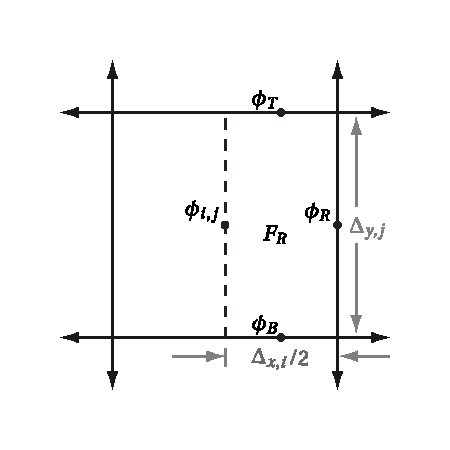
\includegraphics{goldin-righthalf}
  \caption{Right half of cell $i,j$.}
  \label{fig:goldinRight}
\end{figure}
evaluating the flux exiting the right face $F_R^x = \vec{F}\vd\vec{n}_R$.
\begin{align*}
\int_{y_{j-1/2}}^{y_{j+1/2}} \int_{x_{i}}^{x_{i+1/2}}
\vec{n}_R \vd \vec{F}
\ud x \ud y
&=
\int_{y_{j-1/2}}^{y_{j+1/2}} \int_{x_{i}}^{x_{i+1/2}}
-\vec{n}_R \vd \Dtens \vd \grad \phi
\ud x \ud y
\\
F_R^x \frac{\Delta_{x,i} \Delta_{y,j}}{2}
&=
-
\begin{bmatrix}
  1 & 0
\end{bmatrix}
\begin{bmatrix}
  D_{i,j}^{xx} & D_{i,j}^{yx} \\
  D_{i,j}^{xy} & D_{i,j}^{yy}
\end{bmatrix}
\int_{y_{j-1/2}}^{y_{j+1/2}} \int_{x_{i}}^{x_{i+1/2}}
\begin{bmatrix}
  \tpder{\phi}{x} \\
  \tpder{\phi}{y}
\end{bmatrix}
\ud x \ud y
\\
F_R^x \frac{\Delta_{x,i} \Delta_{y,j}}{2}
&=
-
\begin{bmatrix}
  D_{i,j}^{xx} & D_{i,j}^{yx}
\end{bmatrix}
\begin{bmatrix}
  \left( \phi_R - \phi_{i,j} \right) \Delta_{y,j} \\
  \left( \phi_T - \phi_B \right) \Delta_{x,i} / 2
\end{bmatrix}
\ud x \ud y
\\
F_R^x
&= 
- D_{i,j}^{xx} \frac{\phi_R - \phi_{i,j}}{ \Delta_{x,i} / 2}
- D_{i,j}^{yx} \frac{\phi_T - \phi_B}{ \Delta_{y,j} }\ \,.
\end{align*}
Performing the same procedure for the left side, we obtain
\begin{align*}
\int_{y_{j-1/2}}^{y_{j+1/2}} \int_{x_{i-1/2}}^{x_{i}}
\vec{n}_L \vd \vec{F}
\ud x \ud y
&=
\int_{y_{j-1/2}}^{y_{j+1/2}} \int_{x_{i-1/2}}^{x_{i}}
-\vec{n}_L \vd \Dtens \vd \grad \phi
\ud x \ud y
\\
-F_L^x \frac{\Delta_{x,i} \Delta_{y,j}}{2}
&=
-
\begin{bmatrix}
  -1 & 0
\end{bmatrix}
\begin{bmatrix}
  D_{i,j}^{xx} & D_{i,j}^{yx} \\
  D_{i,j}^{xy} & D_{i,j}^{yy}
\end{bmatrix}
\int_{y_{j-1/2}}^{y_{j+1/2}} \int_{x_{i-1/2}}^{x_{i}}
\begin{bmatrix}
  \tpder{\phi}{x} \\
  \tpder{\phi}{y}
\end{bmatrix}
\ud x \ud y
\\
F_L^x \frac{\Delta_{x,i} \Delta_{y,j}}{2}
&=
-
\begin{bmatrix}
  D_{i,j}^{xx} & D_{i,j}^{yx}
\end{bmatrix}
\begin{bmatrix}
  \left( \phi_{i,j} - \phi_L \right) \Delta_{y,j} \\
  \left( \phi_T - \phi_B \right) \Delta_{x,i} / 2
\end{bmatrix}
\ud x \ud y
\\
F_L^x
&= 
- D_{i,j}^{xx} \frac{\phi_{i,j} - \phi_L}{ \Delta_{x,i} / 2}
- D_{i,j}^{yx} \frac{\phi_T - \phi_B}{ \Delta_{y,j} }\,.
\end{align*}

Rotating the coordinate system by swapping $x\leftrightarrow y$, $T
\leftrightarrow R$, $B \leftrightarrow L$, and $i \leftrightarrow j$, we have
corresponding equations for the top and bottom leakage terms:
\begin{align*}
F_T^y
&= 
- D_{i,j}^{yy} \frac{\phi_T - \phi_{i,j}}{ \Delta_{y,j} / 2}
- D_{i,j}^{xy} \frac{\phi_R - \phi_L}{ \Delta_{x,i} }\,,
\\  
F_B^y
&= 
- D_{i,j}^{yy} \frac{\phi_{i,j} - \phi_B}{ \Delta_{y,j} / 2}
- D_{i,j}^{xy} \frac{\phi_R - \phi_L}{ \Delta_{x,i} }\,.
\end{align*}

At each interior face, we demand that the scalar intensity $\phi$ is continuous,
i.e.,
\begin{equation*}
  \phi_{R,i,j} = \phi_{L,i+1,j} \equiv \phi_*\,.
\end{equation*}
Substituting these definitions and the net leakage expressions into the
conservation equation~\eqref{eq:ssConservationDisc}, we obtain $I\times J$
equations,
\begin{multline*}
- \Delta_{x,i} D_{i,j}^{yy}\frac{\phi_{i,j+1/2} - \phi_{i,j}}{\Delta_{y,j} / 2}
- \Delta_{x,i} D_{i,j}^{xy}\frac{\phi_* - \phi_{i-1/2,j}}{\Delta_{x,i} }
\\
+ \Delta_{x,i} D_{i,j}^{yy}\frac{\phi_{i,j} - \phi_{i,j-1/2}}{\Delta_{y,j} / 2}
+ \Delta_{x,i} D_{i,j}^{xy}\frac{\phi_* - \phi_{i-1/2,j}}{\Delta_{x,i} }
\\
- \Delta_{y,j} D_{i,j}^{xx}\frac{\phi_* - \phi_{i,j}}{\Delta_{x,i} / 2}
- \Delta_{y,j} D_{i,j}^{yx}\frac{\phi_{i,j+1/2} - \phi_{i,j-1/2}}{\Delta_{y,j} }
\\
+ \Delta_{y,j} D_{i,j}^{xx}\frac{\phi_{i,j} - \phi_{i-1/2,j}}{\Delta_{x,i} / 2}
+ \Delta_{y,j} D_{i,j}^{yx}\frac{\phi_{i,j+1/2} - \phi_{i,j-1/2}}{\Delta_{y,j} }
\\
+ \Delta_{x,i}\Delta_{y,j} \sigma_{a,i,j} \phi_{i,j}
= \Delta_{x,i}\Delta_{y,j} q_{i,j}\,.
\end{multline*}
The transverse leakage terms cancel, leaving
\begin{multline*}
\phi_{i,j} \left(
   4 D_{i,j}^{xx} \frac{\Delta_{y,j}}{\Delta_{x,i}}
 + 4 D_{i,j}^{yy} \frac{\Delta_{x,i}}{\Delta_{y,j}}
 + \Delta_{x,i}\Delta_{y,j} \sigma_{a,i,j} \right)
 \\
- 2 D_{i,j}^{xx} \frac{\Delta_{y,j}}{\Delta_{x,i}}
  \left( \phi_* + \phi_{i-1/2,j} \right)
- 2 D_{i,j}^{yy} \frac{\Delta_{x,i}}{\Delta_{y,j}}
  \left( \phi_{i,j+1/2} + \phi_{i,j-1/2} \right)
\\= \Delta_{x,i}\Delta_{y,j} q_{i,j}\,.
\end{multline*}

To complete the equations for the Gol'din discretization, we enforce continuity
of the radiation flux on interior faces, setting $F_{T,i,j}^y = F_{B,i,j+1}^y$
and $F_{R,i,j}^x = F_{L,i+1,j}^x$, to yield the relations
\begin{equation*}
- D_{i,j}^{yy} \frac{\phi_{i,j+1/2} - \phi_{i,j}}{ \Delta_{y,j} / 2}
- D_{i,j}^{xy} \frac{\phi_* - \phi_{i-1/2,j}}{ \Delta_{x,i} }
=
- D_{i,j+1}^{yy} \frac{\phi_{i,j+1} - \phi_{i,j+1/2}}{ \Delta_{y,j} / 2}
- D_{i,j+1}^{xy} \frac{\phi_{i+1/2,j+1} - \phi_{i-1/2,j+1}}{ \Delta_{x,i} }\,.
\end{equation*}
and
\begin{equation*}
- D_{i,j}^{xx} \frac{\phi_* - \phi_{i,j}}{ \Delta_{x,i} / 2}
- D_{i,j}^{yx} \frac{\phi_{i,j+1/2} - \phi_{i,j-1/2}}{ \Delta_{y,j} }
=
- D_{i+1,j}^{xx} \frac{\phi_{i+1,j} - \phi_{i,j}}{ \Delta_{x,i} / 2}
- D_{i+1,j}^{yx} \frac{\phi_{i+1,j+1/2} - \phi_{i+1,j-1/2}}{ \Delta_{y,j} }\,.
\end{equation*}

Note that, if $D^{xy} = D^{yx}=0$, the cell-edged $\phi$ can be eliminated
without approximation, and
Gol'din's method will reduce to the simple cell-centered difference scheme of
\S\ref{sec:discreteDiag}.

%%%%%%%%%%%%%%%%%%%%%%%%%%%%%%%%%%%%%%%%%%%%%%%%%%%%%%%%%%%%%%%%%%%%%%%%%%%%%%%%
\section{Nine-point stencil}

Fig.~\ref{fig:cellAnisoLeakage} shows the leakage out of cell $i,j$ through the
right face.
\begin{figure}[htb]
  \centering
  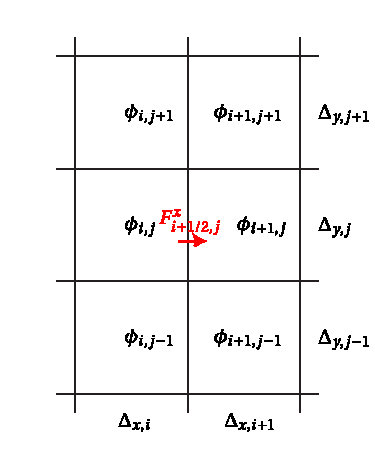
\includegraphics{cell-leakage-right}
  \caption{Diagram showing the radiation exiting interior cell $i,j$ through the
  right face.}
  \label{fig:cellAnisoLeakage}
\end{figure}
We evaluate the face-averaged normal component of the flux,
$F_{i+1/2,j}^x \equiv \int_{y_{j-1/2}}^{y_{j+1/2}} \vec{F} \vd \vec{n} \ud
y$, from both cell $i,j$ and cell $i+1,j$, and set them equal to each other.
Solving for $F_{i+1/2,j}^x$ gives
\begin{equation} \label{eq:cellAnisoFlux}
  F_{i+1/2,j}^{x} \approx
  - \frac{D^{xx}_{i+1/2,j}}{\Delta_{x,i+1/2}}
  \left[ 
    \left( \phi_{i+1,j} - \phi_{i,j} \right)
  + \frac{D^{xy}_{i,j}/D^{xx}_{i,j}}{2/\Delta_{x,i}}
    \pder{\phi}{y} \Bigg|_{x_{i+1/2}^-}
  + \frac{D^{xy}_{i+1,j}/D^{xx}_{i+1,j}}{2/\Delta_{x,i+1}}
    \pder{\phi}{y} \Bigg|_{x_{i+1/2}^+}
  \right]
\end{equation}
where $\tpder{\phi}{y} |_{x_{i+1/2}^-}$ is the transverse derivative of
$\phi$ on the left side of the face, and $\tpder{\phi}{y} |_{x_{i+1/2}^+}$ is
the transverse derivative as viewed from the right side of the face.
The harmonic-averaged diffusion coefficient is
\begin{equation} \tagref{eq:cellEdgeDHarmonic}
  \frac{D^{xx}_{i+1/2,j}}{\Delta_{x,i+1/2}} \equiv \left[
  \frac12 \left( \frac{D^{xx}_{i,j}}{\Delta_{x,i}} \right)\inv
 + \frac12 \left( \frac{D^{xx}_{i+1,j}}{\Delta_{x,i+1}} \right)\inv
  \right]\inv\,.
\end{equation}

If $D^{xy}$ were zero for both cells, and $D^{xx}=D^{yy}$,
Eq.~\eqref{eq:cellAnisoFlux} would reduce to
the standard cell-centered finite difference discretization so well known to
nuclear engineering students.

Now, in our first nine-point stencil, we approximated
\begin{equation*}
  \pder{\phi}{y} \Bigg|_{x_{i+1/2}^-} \approx \frac{\phi_{i,j+1} -
  \phi_{i,j-1}}{\tfrac12 \Delta_{y,j+1} + \Delta_{y,j} + \tfrac12
  \Delta_{y,j-1}}
\end{equation*}
in the interior of the problem and discarded the term near the boundaries. (The 
$\tpder{\phi}{y} |_{x_{i+1/2}^+}$ term is the same but replacing $i\to i+1$.)
An improvement is to approximate the case on the top boundary with
\begin{equation*}
  \pder{\phi}{y} \Bigg|_{x_{i+1/2}^-} \approx \frac{\phi_{i,j} -
  \phi_{i,j-1}}{\tfrac12 \Delta_{y,j} + \tfrac12 \Delta_{y,j-1} }
\end{equation*}
and the case on the bottom boundary with 
\begin{equation*}
  \pder{\phi}{y} \Bigg|_{x_{i+1/2}^-} \approx \frac{\phi_{i,j+1} -
  \phi_{i,j}}{\tfrac12 \Delta_{y,j+1} + \tfrac12 \Delta_{y,j} }
\end{equation*}

We can also approximate this derivative with approximate cell-edge values. In
the finite difference method, an intermediate cell-edge $\phi$ helps represent
the slope normal to the edge. It is eliminated in the process of finding
$\vec{F}\vd\vec{n}$, but if there is no transverse term, it is possible to
solve for the cell-edge $\phi$ in terms of the two cell-centered $\phi$. Let us
consider the finite difference approximation coupling two cells:
\begin{equation*}
  F = - D_0 \frac{\phi_{1/2} - \phi_0}{\Delta_0/2}
  \qquad\text{and}\qquad
  F = - D_1 \frac{\phi_{1} - \phi_{1/2}}{\Delta_1/2}\,.
\end{equation*}
Multiplying the left equation by $\Delta_0 / D_0$ and the right equation by
$\Delta_1 / D_1$,
\begin{equation*}
  -\frac{\Delta_0/2}{D_0 } F = \phi_{1/2} - \phi_0
  \qquad\text{and}\qquad
  -\frac{\Delta_1/2}{D_1 } F = \phi_{1} - \phi_{1/2}
\end{equation*}
adding them eliminates gives the standard finite-difference approximation for
$F$,
\begin{equation*}
  F = - \left( \frac{\Delta_0/2}{D_0 } + \frac{\Delta_1/2}{D_1 } \right)\inv
  \left( \phi_1 - \phi_0 \right),
\end{equation*}
and subtracting the second from the first gives
\begin{equation*}
 -\frac{\Delta_0/2}{D_0 }F + \frac{\Delta_1/2}{D_1 } F
 = 2 \phi_{1/2}-(\phi_0+\phi_1)\,.
\end{equation*}
Defining $ d_i \equiv \frac{\Delta_i}{D_i}$ for $i=0,1$ for brevity, then
\begin{equation*}
  \frac12 F (d_1 - d_0)
 = 2 \phi_{1/2}-(\phi_0+\phi_1)
  \qquad\text{and}\qquad
 F = -2\left( d_1 + d_0 \right)\inv (\phi_1 - \phi_0)\,.
\end{equation*}
Substituting $F$ into the left equation,
\begin{align*}
  \left( d_1 + d_0 \right)\inv\left(d_1 - d_0\right) (\phi_1 - \phi_0)
  &= 2 \phi_{1/2}-(\phi_0+\phi_1)
  \\
 \frac12 \left[ 1 - \frac{d_1 - d_0}{d_1 + d_0} \right] \phi_1
+ \frac12 \left[ 1 + \frac{d_1 - d_0}{d_1 + d_0} \right] \phi_0
 &= \phi_{1/2}
  \\
 \frac{d_0}{d_1 + d_0} \phi_1
+ \frac{d_1}{d_1 + d_0} \phi_0
 &= \phi_{1/2}\,.
\end{align*}

For our case in anisotropic diffusion, we want to approximate 
\begin{equation*}
  \pder{\phi}{y} \Bigg|_{x_{i+1/2}^-} \approx \frac{\phi_{i,j+1/2} -
  \phi_{i,j-1/2}}{\Delta_{y,j}} \,.
\end{equation*}
In evaluating these cell-edge $\phi$ we neglect the transverse leakage (as
leaving them in would add unknowns on more cell faces) and apply the previous
result:
\begin{equation*}
  \phi_{i,j+1/2} \approx
  \frac{D_{i,j}^{yy} / \Delta_{y,j}}{D_{i,j+1}^{yy} / \Delta_{y,j+1} +
  D_{i,j}^{yy} / \Delta_{y,j}} \phi_{i,j+1}
+ \frac{D_{i,j+1}^{yy} / \Delta_{y,j+1}}{D_{i,j+1}^{yy} / \Delta_{y,j+1} +
D_{i,j}^{yy} / \Delta_{y,j}} \phi_{i,j} \,.
\end{equation*}
Subtracting one from the $j$ indices gives the corresponding equation for the
bottom face:
\begin{equation*}
  \phi_{i,j-1/2} \approx
  \frac{D_{i,j-1}^{yy} / \Delta_{y,j-1}}{D_{i,j}^{yy} / \Delta_{y,j} +
  D_{i,j-1}^{yy} / \Delta_{y,j-1}} \phi_{i,j}
+ \frac{D_{i,j}^{yy} / \Delta_{y,j}}{D_{i,j}^{yy} / \Delta_{y,j} +
D_{i,j-1}^{yy} / \Delta_{y,j-1}} \phi_{i,j-1} \,.
\end{equation*}
If cell $i,j$ is in the interior, 
\begin{equation*}
  \pder{\phi}{y} \Bigg|_{x_{i+1/2}^-} \approx \frac{\phi_{i,j+1/2} -
  \phi_{i,j-1/2}}{\Delta_{y,j}} \,,
\end{equation*}
or if it is on the top boundary,
\begin{equation*}
  \pder{\phi}{y} \Bigg|_{x_{i+1/2}^-} \approx \frac{\phi_{i,j} -
  \phi_{i,j-1/2}}{\Delta_{y,j} / 2} \,,
\end{equation*}
or if it is on the bottom boundary,
\begin{equation*}
  \pder{\phi}{y} \Bigg|_{x_{i+1/2}^-} \approx \frac{\phi_{i,j+1/2} -
  \phi_{i,j}}{\Delta_{y,j} / 2} \,.
\end{equation*}

If the anisotropic diffusion coefficients are homogeneous and the grid is
uniform, this expression for $\tpder{\phi}{y}$ is exactly equivalent to the
simpler one.

\begin{figure}[htb]
  \centering
  \subfloat[Diagonal-only anisotropic]{%
  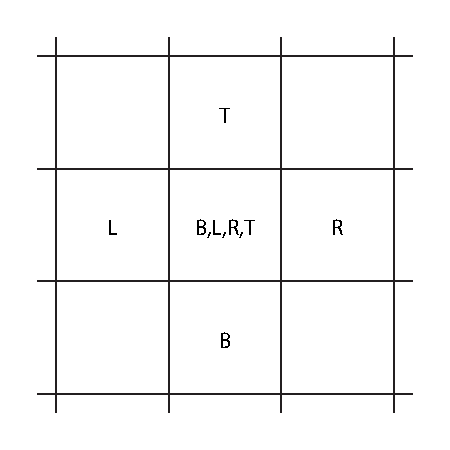
\includegraphics{diaganiso-leakage-terms}}
  \subfloat[Cell anisotropic]{%
  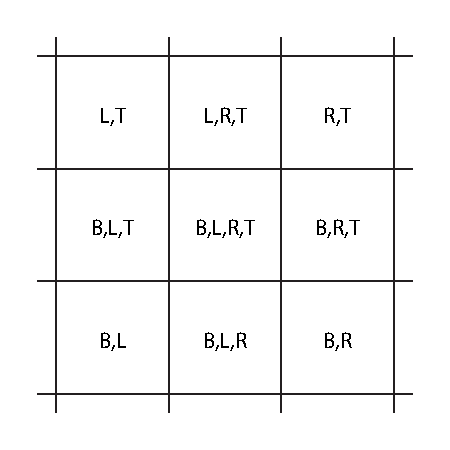
\includegraphics{cellaniso-leakage-terms}}
  \caption{Stencils for $- \grad \vd \Dtens \grad \phi$ showing contribution
  from the leakage terms of each face of the center cell.}
  \label{fig:anisoStencils}
\end{figure}

